\documentclass[conference]{./common/IEEEtran}


\usepackage{listings} % source code
\usepackage{pdfpages} % pdf
\usepackage{cite}     % for bibtext
\usepackage{url}      % url
\usepackage{pgfplots} % plot
\usepackage{hyperref}


\hyphenation{op-tical net-works semi-conduc-tor}
\begin{document}
\title{Evaluation for Viki.com}
\author{
\IEEEauthorblockN{Kamol Mavlonov}
\{{kamoljan\}@gmail.com}
}

\maketitle

\begin{abstract}
To improve user experience we are looking for the ways to improve performance of Viki.com.
\end{abstract}

\section{Introduction}
All evaluations in this document are for Viki.com performance improvement. 

\subsection{Requirement tools for these evaluations}
Mobile network enabled device. It can be mobile broadband or tethering enabled mobile device.
Need a laptop with installed {siege}[1] and {ab}[4]. Siege is an http load testing and benchmarking utility. 
It was designed to let web developers measure their code under duress, to see how it will stand up to load on the Internet. 
Siege supports basic authentication, cookies, HTTP and HTTPS protocols. 
It lets its user hit a web server with a configurable number of simulated web browsers.
Moreover, additional evaluation results are taking from Google {pagespeed}[2] and Yahoo {yslow}[3]

\section{Evaluation}
\pgfplotsset{}

\begin{figure}[ht]
\begin{minipage}[b]{\linewidth}\centering
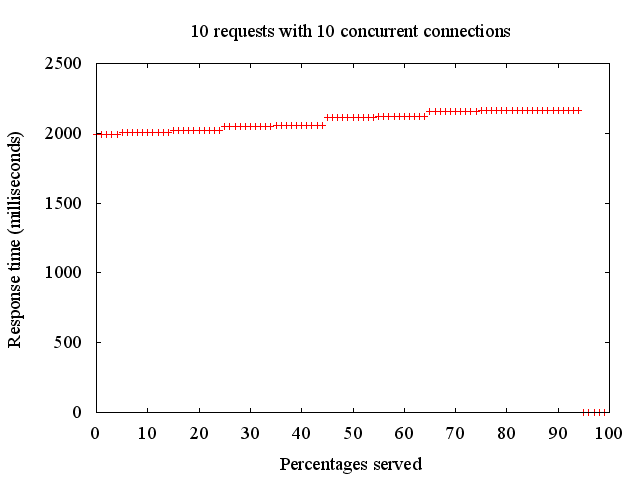
\includegraphics[width=\textwidth]{include/gnu/10_10.png}
\end{minipage}
\caption{10 requests with 10 concurrent connections.}
\label{fig:my_read_latency}
\end{figure}

\begin{figure}[ht]
\begin{minipage}[b]{\linewidth}\centering
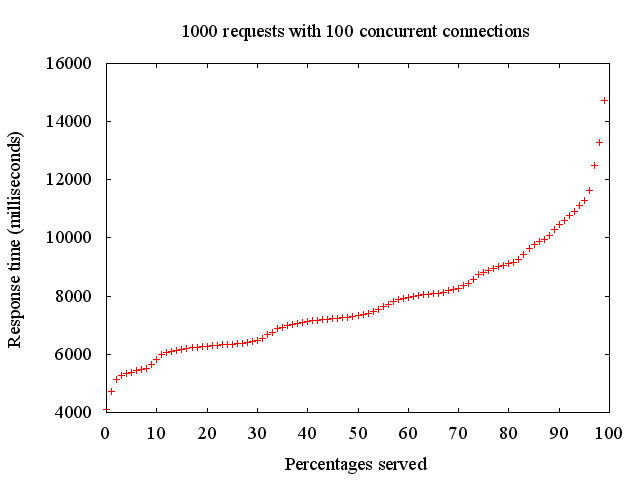
\includegraphics[width=\textwidth]{include/gnu/1000_100.png}
\end{minipage}
\caption{1000 request with 100 concurrent connections.}
\label{fig:my_read_latency}
\end{figure}

\section{Conclusion} 

\section{Acknowledgment}
The authors would like to thank Viki team for their hard work.

\begin{thebibliography}{1}
\bibitem{IEEEhowto:siege}
http://www.joedog.org/siege-home/
\bibitem{IEEEhowto:pagespeed}
https://developers.google.com/speed/pagespeed/
\bibitem{IEEEhowto:yslow}
http://developer.yahoo.com/yslow/
\bibitem{IEEEhowto:ab}
http://httpd.apache.org/docs/2.2/programs/ab.html
\end{thebibliography}

\end{document}


